\documentclass[12pt,letterpaper]{article}\usepackage[]{graphicx}\usepackage[]{color}
%% maxwidth is the original width if it is less than linewidth
%% otherwise use linewidth (to make sure the graphics do not exceed the margin)
\makeatletter
\def\maxwidth{ %
  \ifdim\Gin@nat@width>\linewidth
    \linewidth
  \else
    \Gin@nat@width
  \fi
}
\makeatother

\definecolor{fgcolor}{rgb}{0.345, 0.345, 0.345}
\newcommand{\hlnum}[1]{\textcolor[rgb]{0.686,0.059,0.569}{#1}}%
\newcommand{\hlstr}[1]{\textcolor[rgb]{0.192,0.494,0.8}{#1}}%
\newcommand{\hlcom}[1]{\textcolor[rgb]{0.678,0.584,0.686}{\textit{#1}}}%
\newcommand{\hlopt}[1]{\textcolor[rgb]{0,0,0}{#1}}%
\newcommand{\hlstd}[1]{\textcolor[rgb]{0.345,0.345,0.345}{#1}}%
\newcommand{\hlkwa}[1]{\textcolor[rgb]{0.161,0.373,0.58}{\textbf{#1}}}%
\newcommand{\hlkwb}[1]{\textcolor[rgb]{0.69,0.353,0.396}{#1}}%
\newcommand{\hlkwc}[1]{\textcolor[rgb]{0.333,0.667,0.333}{#1}}%
\newcommand{\hlkwd}[1]{\textcolor[rgb]{0.737,0.353,0.396}{\textbf{#1}}}%

\usepackage{framed}
\makeatletter
\newenvironment{kframe}{%
 \def\at@end@of@kframe{}%
 \ifinner\ifhmode%
  \def\at@end@of@kframe{\end{minipage}}%
  \begin{minipage}{\columnwidth}%
 \fi\fi%
 \def\FrameCommand##1{\hskip\@totalleftmargin \hskip-\fboxsep
 \colorbox{shadecolor}{##1}\hskip-\fboxsep
     % There is no \\@totalrightmargin, so:
     \hskip-\linewidth \hskip-\@totalleftmargin \hskip\columnwidth}%
 \MakeFramed {\advance\hsize-\width
   \@totalleftmargin\z@ \linewidth\hsize
   \@setminipage}}%
 {\par\unskip\endMakeFramed%
 \at@end@of@kframe}
\makeatother

\definecolor{shadecolor}{rgb}{.97, .97, .97}
\definecolor{messagecolor}{rgb}{0, 0, 0}
\definecolor{warningcolor}{rgb}{1, 0, 1}
\definecolor{errorcolor}{rgb}{1, 0, 0}
\newenvironment{knitrout}{}{} % an empty environment to be redefined in TeX

\usepackage{alltt}
 \usepackage[left=2cm,right=2cm,top=2cm,bottom=2cm]{geometry}
\usepackage[ansinew]{inputenc}
\usepackage[spanish]{babel}
\usepackage{amsmath}
\usepackage{amsfonts}
\usepackage{amssymb}
\usepackage{dsfont}
\usepackage{multicol} 
\usepackage{subfigure}
\usepackage{graphicx}
\usepackage{float} 
\usepackage{verbatim} 
\usepackage[left=2cm,right=2cm,top=2cm,bottom=2cm]{geometry}
\usepackage{fancyhdr}
\pagestyle{fancy} 
\fancyhead[LO]{\leftmark}
\usepackage{caption}
\newtheorem{definicion}{Definci\'on}
\IfFileExists{upquote.sty}{\usepackage{upquote}}{}
\begin{document}

\begin{titlepage}
\setlength{\unitlength}{1 cm} %Especificar unidad de trabajo

\begin{center}
\textbf{{\large UNIVERSIDAD DE EL SALVADOR}\\ [0.50 cm]
{\large FACULTAD MULTIDISCIPLINARIA DE OCCIDENTE}\\ [0.50 cm]
{\large DEPARTAMENTO DE MATEM\'ATICA}}\\ [0.50 cm]

\begin{picture}(18,4)
 \put(7,0){
\includegraphics[width=4cm]{minerva.jpg}}
\end{picture}
\\ [0.25 cm]

\textbf{{\large Licenciatura en Estad\'istica}\\ [1.25cm]
{\large Control Estad\'istico del Paquete R }\\ [2 cm]
%\setlength{\unitlength}{1 cm}
{\large  \textbf{"UNIDAD DOS"}}\\ [3 cm]
{\large Alumna:}\\
{\large Erika Beatr\'iz Guill\'en Pineda}\\ [2cm]
{\large Fecha de elaboraci\'on}\\
Santa Ana - \today }
\end{center}
\end{titlepage}

\newtheorem{teorema}{Teorema}
\newtheorem{prop}{Proposici\'on}[section]

\lhead{Pr\'actica 06}

\lfoot{LICENCIATURA EN ESTAD\'ISTICA}
\cfoot{UESOCC}
\rfoot{\thepage}
%\pagestyle{fancy} 

\setcounter{page}{1}
\newpage
\section{ESCALAS DE MEDICI\'ON} 

Los tipos de datos univariados que vamos a analizar en esta pr\'actica son:

\textbf{Categ\'iricos:} Tienen la caracter\'istica de que todos los miembros de una categor\'ia se consideran
iguales en lo que se refiere a ese tipo. Este tipo de datos se subdivide en nominales y ordinales.

\textbf{Nominales:}Los valores que pueden asumir sirven para clasificarlos pero no para
ordenarlos. En caso de usarse n?meros, s\'olo se adoptan como nombres o identificaciones.

\textbf{Ordinales:} Los valores que puede asumir este tipo de datos son categor?as que conllevan un juicio de valor que exige comparar a los diferentes elementos de la muestra con respecto a este tipo con el objeto de establecer un orden. Es decir, que los datos se organizan a trav\'es de las relaciones de igualdad, mayor o menor.

\subsection{AN\'ALISIS ESTAD?STICO DE DATOS CATEG\'ORICOS}  

Ejemplo: Se realiza un estudio para conocer las preferencias sobre el tipo de gaseosa que se
consume: "CC"=Coca Cola, "PC"=Pepsi Cola, "SC"=Salva Cola, para ello se toma una muestra
aleatoria de 20 personas

1) Activar el directorio de trabajo
\begin{knitrout}
\definecolor{shadecolor}{rgb}{0.969, 0.969, 0.969}\color{fgcolor}\begin{kframe}
\begin{alltt}
\hlkwd{getwd}\hlstd{()}
\end{alltt}
\begin{verbatim}
## [1] "C:/Users/User/Documents/TODAS_PRACTICAS"
\end{verbatim}
\begin{alltt}
\hlkwd{setwd}\hlstd{(}\hlstr{"C:/Users/User/Documents/TODAS_PRACTICAS"}\hlstd{)}
\end{alltt}
\end{kframe}
\end{knitrout}

2) Crear un nuevo script y llamarle Script06-DatosCategoricos


3) Crear un vector con el tipo de gaseosa y otro con la muestra generada aleatoriamente:
\begin{knitrout}
\definecolor{shadecolor}{rgb}{0.969, 0.969, 0.969}\color{fgcolor}\begin{kframe}
\begin{alltt}
\hlstd{Tipo} \hlkwb{<-} \hlkwd{c}\hlstd{(}\hlstr{"CC"}\hlstd{,} \hlstr{"PC"}\hlstd{,} \hlstr{"SC"}\hlstd{);}
\hlstd{Tipo} \hlcom{# crea un vector en las que contiene los tres tipos de refrescos}
\end{alltt}
\begin{verbatim}
## [1] "CC" "PC" "SC"
\end{verbatim}
\begin{alltt}
\hlstd{Consumo} \hlkwb{<-} \hlkwd{sample}\hlstd{(Tipo,} \hlnum{20}\hlstd{,} \hlkwc{replace}\hlstd{=}\hlnum{TRUE}\hlstd{);}
\hlstd{Consumo}
\end{alltt}
\begin{verbatim}
##  [1] "CC" "PC" "PC" "SC" "PC" "CC" "PC" "CC" "CC" "PC" "SC" "SC" "PC" "PC"
## [15] "CC" "CC" "SC" "PC" "SC" "PC"
\end{verbatim}
\begin{alltt}
\hlcom{# genera una muestra de tama?o 20 obtenida de los elementos del vector Tipo }
\hlcom{# y los elementos se seleccionan con reemplazamiento}

\hlcom{# Suponiendo que se quiere editar o agregar datos}
\hlkwd{data.entry}\hlstd{(Consumo)}
\end{alltt}
\end{kframe}
\end{knitrout}

4) Guarde el vector en un archivo de datos
\begin{knitrout}
\definecolor{shadecolor}{rgb}{0.969, 0.969, 0.969}\color{fgcolor}\begin{kframe}
\begin{alltt}
\hlcom{# Guardar los datos en su directorio de trabajo}
\hlkwd{write}\hlstd{(Consumo,} \hlstr{"Consumo.txt"}\hlstd{)}
\end{alltt}
\end{kframe}
\end{knitrout}

5) Eliminar los objetos que existen en el espacio de trabajo (Workspace)
\begin{knitrout}
\definecolor{shadecolor}{rgb}{0.969, 0.969, 0.969}\color{fgcolor}\begin{kframe}
\begin{alltt}
\hlkwd{ls}\hlstd{()}
\end{alltt}
\begin{verbatim}
## [1] "Consumo" "Tipo"
\end{verbatim}
\begin{alltt}
\hlkwd{rm}\hlstd{(}\hlkwc{list}\hlstd{=}\hlkwd{ls}\hlstd{(}\hlkwc{all}\hlstd{=}\hlnum{TRUE}\hlstd{))}
\hlkwd{ls}\hlstd{()}
\end{alltt}
\begin{verbatim}
## character(0)
\end{verbatim}
\end{kframe}
\end{knitrout}

6) Leer o recuperar el vector de datos o archivo de texto
\begin{knitrout}
\definecolor{shadecolor}{rgb}{0.969, 0.969, 0.969}\color{fgcolor}\begin{kframe}
\begin{alltt}
\hlstd{Consumo} \hlkwb{<-} \hlkwd{scan}\hlstd{(}\hlstr{"Consumo.txt"}\hlstd{,} \hlkwc{what} \hlstd{=} \hlkwd{character}\hlstd{(),} \hlkwc{na.strings} \hlstd{=} \hlstr{"NA"}\hlstd{,}\hlkwc{flush}\hlstd{=}\hlnum{FALSE}\hlstd{);}
\hlstd{Consumo}
\end{alltt}
\begin{verbatim}
##  [1] "CC" "PC" "PC" "SC" "PC" "CC" "PC" "CC" "CC" "PC" "SC" "SC" "PC" "PC"
## [15] "CC" "CC" "SC" "PC" "SC" "PC"
\end{verbatim}
\begin{alltt}
\hlkwd{ls}\hlstd{()}
\end{alltt}
\begin{verbatim}
## [1] "Consumo"
\end{verbatim}
\begin{alltt}
\hlcom{# Si el vector contiene caracteres se ocupa: what = character()}
\hlcom{# na.strings ="NA", le indica a R que los valores faltantes son identificados con "NA"}
\end{alltt}
\end{kframe}
\end{knitrout}

7) Crear la tabla de distribuci\'on de frecuencias y proporciones
\begin{knitrout}
\definecolor{shadecolor}{rgb}{0.969, 0.969, 0.969}\color{fgcolor}\begin{kframe}
\begin{alltt}
\hlstd{frec} \hlkwb{<-} \hlkwd{table}\hlstd{(Consumo);}
\hlstd{frec}
\end{alltt}
\begin{verbatim}
## Consumo
## CC PC SC 
##  6  9  5
\end{verbatim}
\begin{alltt}
\hlstd{prop} \hlkwb{<-} \hlkwd{table}\hlstd{(Consumo)}\hlopt{/}\hlkwd{length}\hlstd{(Consumo);}
\hlstd{prop}
\end{alltt}
\begin{verbatim}
## Consumo
##   CC   PC   SC 
## 0.30 0.45 0.25
\end{verbatim}
\begin{alltt}
\hlcom{# Note que la salida por defecto no es para nada atractiva en comparaci?n }
\hlcom{# con el resto de paquetes estad\textbackslash{}'isticos.En cambio, si estamos usando }
\hlcom{# LATEX y queremos incorporar estos cuadros o cualquier otro podemos utilizar }
\hlcom{# el comando xtable(table(Consumo)) (NOTE QUE EL ARGUMENTO DEBE SER UN CUADRO), }
\hlcom{# y con esto autom\textbackslash{}'aticamente se nos genera el c\textbackslash{}'odigo en LATEX y luego }
\hlcom{#incorporarlo a nuestro informe, lo mejor de todo es que salida }
\hlcom{# resultante es mucho m\textbackslash{}'as presentable.}
\end{alltt}
\end{kframe}
\end{knitrout}

8) Conocer un resumen de los datos
\begin{knitrout}
\definecolor{shadecolor}{rgb}{0.969, 0.969, 0.969}\color{fgcolor}\begin{kframe}
\begin{alltt}
\hlkwd{summary}\hlstd{(Consumo)}
\end{alltt}
\begin{verbatim}
##    Length     Class      Mode 
##        20 character character
\end{verbatim}
\begin{alltt}
\hlcom{# note que por tratarse de variables cualitativas ?nicamente }
\hlcom{# muestra el n?mero de elementos, y el tipo de datos.}
\end{alltt}
\end{kframe}
\end{knitrout}

9) Realizar un gr?fico de barras
\begin{knitrout}
\definecolor{shadecolor}{rgb}{0.969, 0.969, 0.969}\color{fgcolor}\begin{kframe}
\begin{alltt}
\hlcom{# Para las frecuencias absolutas}
\hlkwd{barplot}\hlstd{(frec,} \hlkwc{main}\hlstd{=}\hlstr{"Gr\textbackslash{}'afico de barras"}\hlstd{,} \hlkwc{xlab}\hlstd{=}\hlstr{" Consumo"}\hlstd{,}
        \hlkwc{col}\hlstd{=}\hlkwd{c}\hlstd{(}\hlstr{"yellow"}\hlstd{,} \hlstr{"purple"}\hlstd{,} \hlstr{"red"}\hlstd{),}\hlkwc{sub}\hlstd{=}\hlstr{"Agosto-2012"}\hlstd{)}
\end{alltt}
\end{kframe}
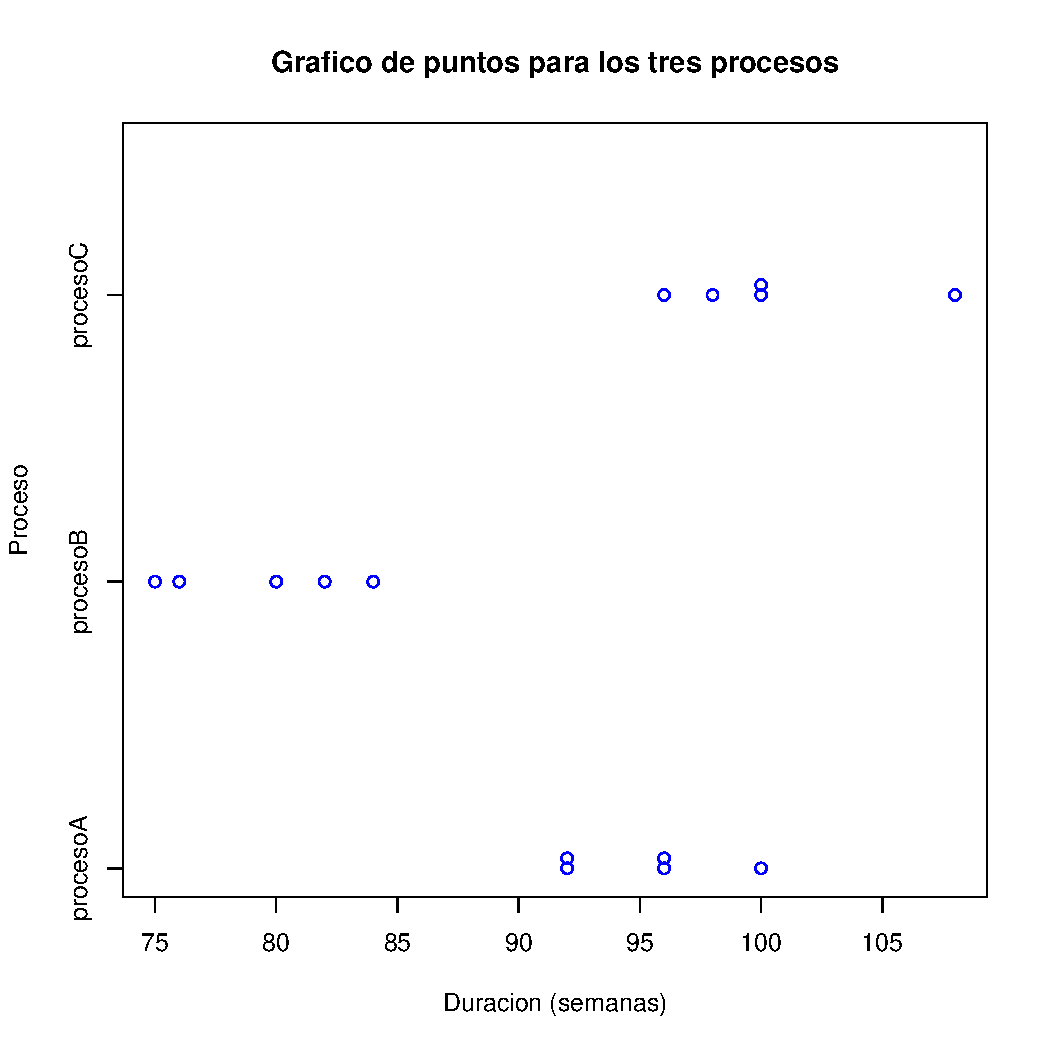
\includegraphics[width=\maxwidth]{figure/unnamed-chunk-8-1} 
\begin{kframe}\begin{alltt}
\hlcom{# Para las frecuencias relativas}
\hlkwd{barplot}\hlstd{(prop,} \hlkwc{main}\hlstd{=}\hlstr{"Gr\textbackslash{}'afico de barras"}\hlstd{,} \hlkwc{xlab}\hlstd{=}\hlstr{" Consumo\textbackslash{}n"}\hlstd{,}
        \hlkwc{col}\hlstd{=}\hlkwd{c}\hlstd{(}\hlstr{"yellow"}\hlstd{,} \hlstr{"purple"}\hlstd{,}\hlstr{"red"}\hlstd{),} \hlkwc{sub}\hlstd{=}\hlstr{"Agosto-2012"}\hlstd{)}
\end{alltt}
\end{kframe}
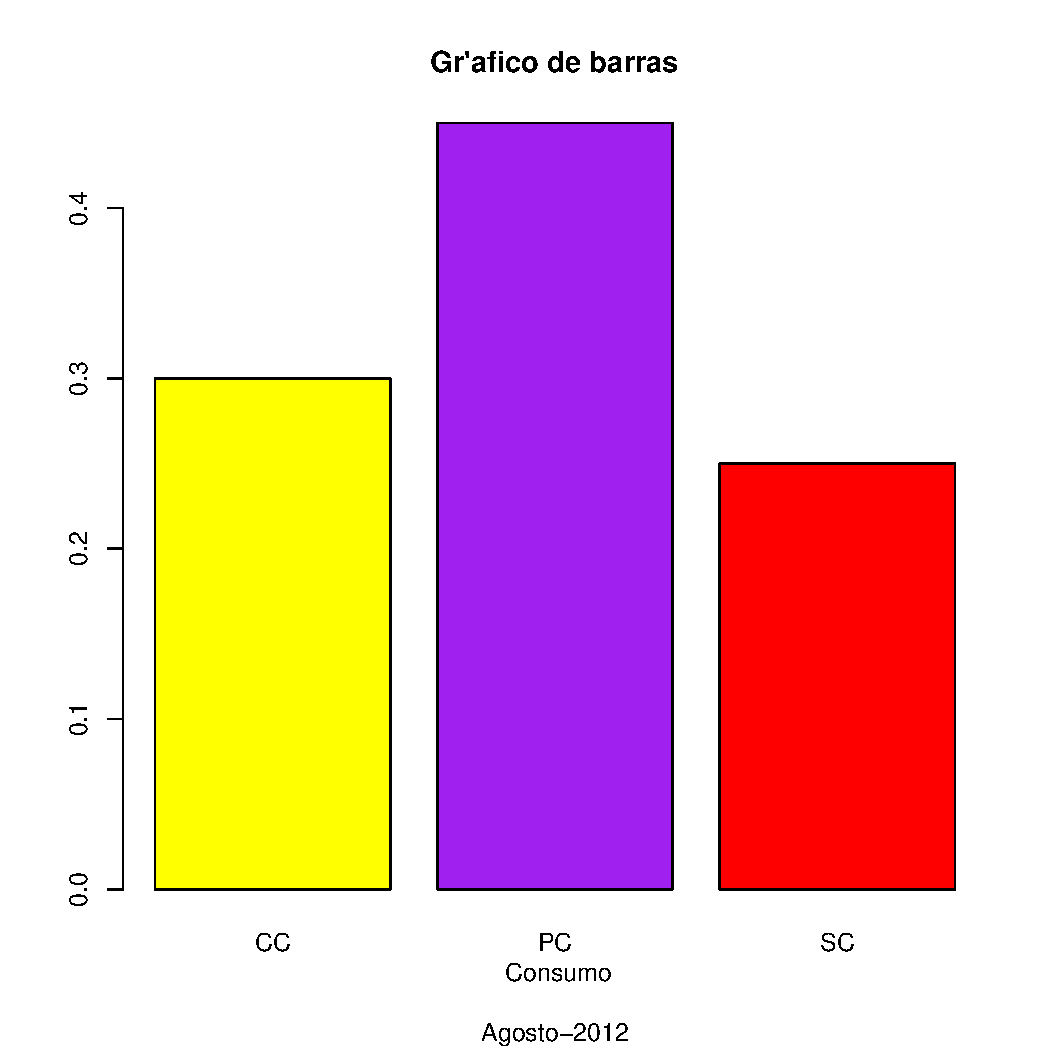
\includegraphics[width=\maxwidth]{figure/unnamed-chunk-8-2} 

\end{knitrout}

10) Realizar un gr\'afico de pastel
\begin{knitrout}
\definecolor{shadecolor}{rgb}{0.969, 0.969, 0.969}\color{fgcolor}\begin{kframe}
\begin{alltt}
\hlkwd{pie}\hlstd{(frec,} \hlkwc{main}\hlstd{=}\hlstr{"Gr\textbackslash{}'afico de pastel"}\hlstd{,} \hlkwc{xlab}\hlstd{=}\hlstr{"Tipo de Consumo"}\hlstd{,}
    \hlkwc{col}\hlstd{=}\hlkwd{c}\hlstd{(}\hlstr{"yellow"}\hlstd{,} \hlstr{"purple"}\hlstd{,}\hlstr{"cyan"}\hlstd{),} \hlkwc{sub}\hlstd{=}\hlstr{"Agosto-2012"}\hlstd{)}
\end{alltt}
\end{kframe}
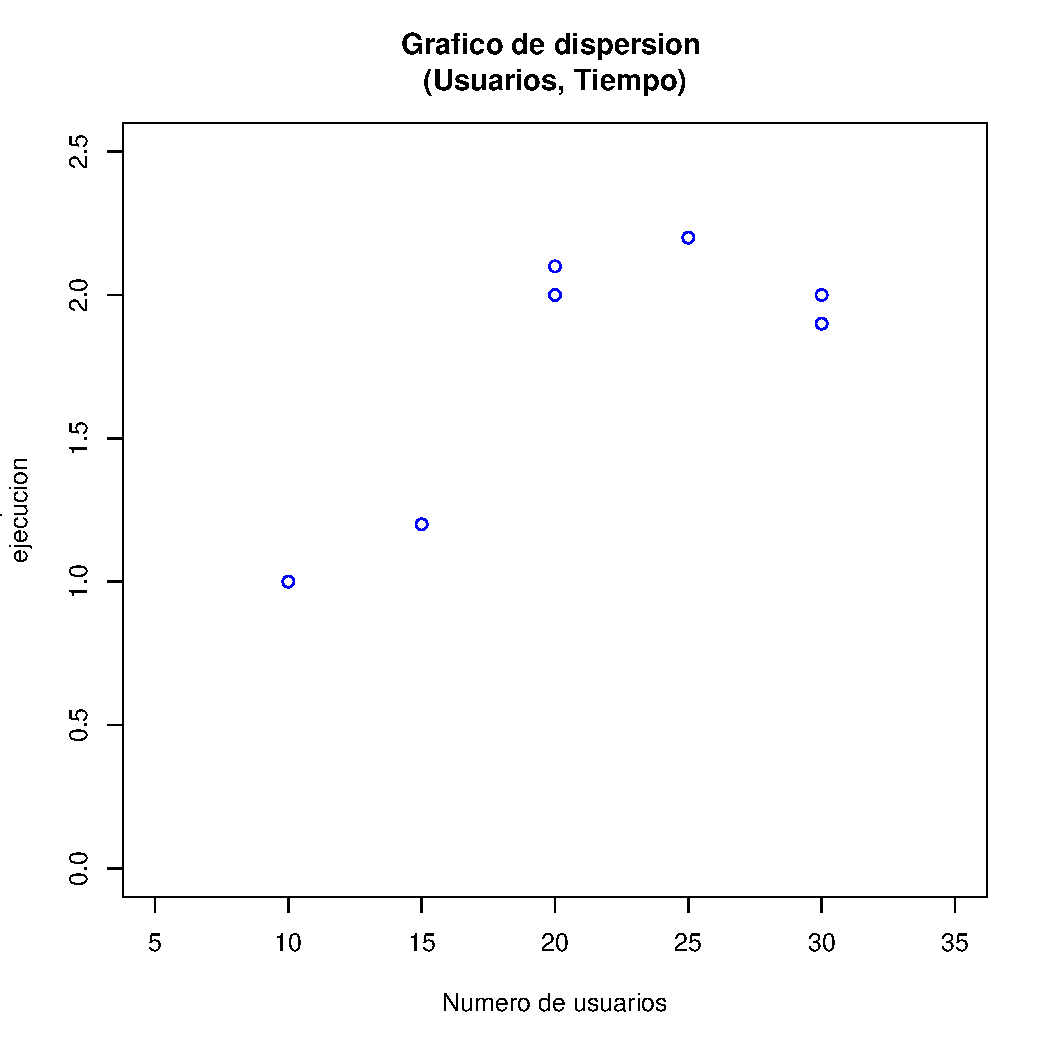
\includegraphics[width=\maxwidth]{figure/unnamed-chunk-9-1} 
\begin{kframe}\begin{alltt}
\hlcom{# Se puede especificar nombres para las categor?as y el color de los sectores}
\hlkwd{names}\hlstd{(frec)} \hlkwb{=} \hlkwd{c}\hlstd{(}\hlstr{"Coca Cola"}\hlstd{,} \hlstr{"Pepsi"}\hlstd{,} \hlstr{"Salva Cola"}\hlstd{)}
\hlkwd{pie}\hlstd{(frec,} \hlkwc{main}\hlstd{=}\hlstr{"Gr\textbackslash{}'afico de pastel"}\hlstd{,} \hlkwc{xlab}\hlstd{=}\hlstr{" Consumo"}\hlstd{,} \hlkwc{radius}\hlstd{=}\hlnum{0.8}\hlstd{,}
    \hlkwc{col}\hlstd{=}\hlkwd{c}\hlstd{(}\hlstr{"red"}\hlstd{,} \hlstr{"gray"}\hlstd{,}\hlstr{"cyan"}\hlstd{),} \hlkwc{sub}\hlstd{=}\hlstr{"Agosto-2012"}\hlstd{)}
\end{alltt}
\end{kframe}
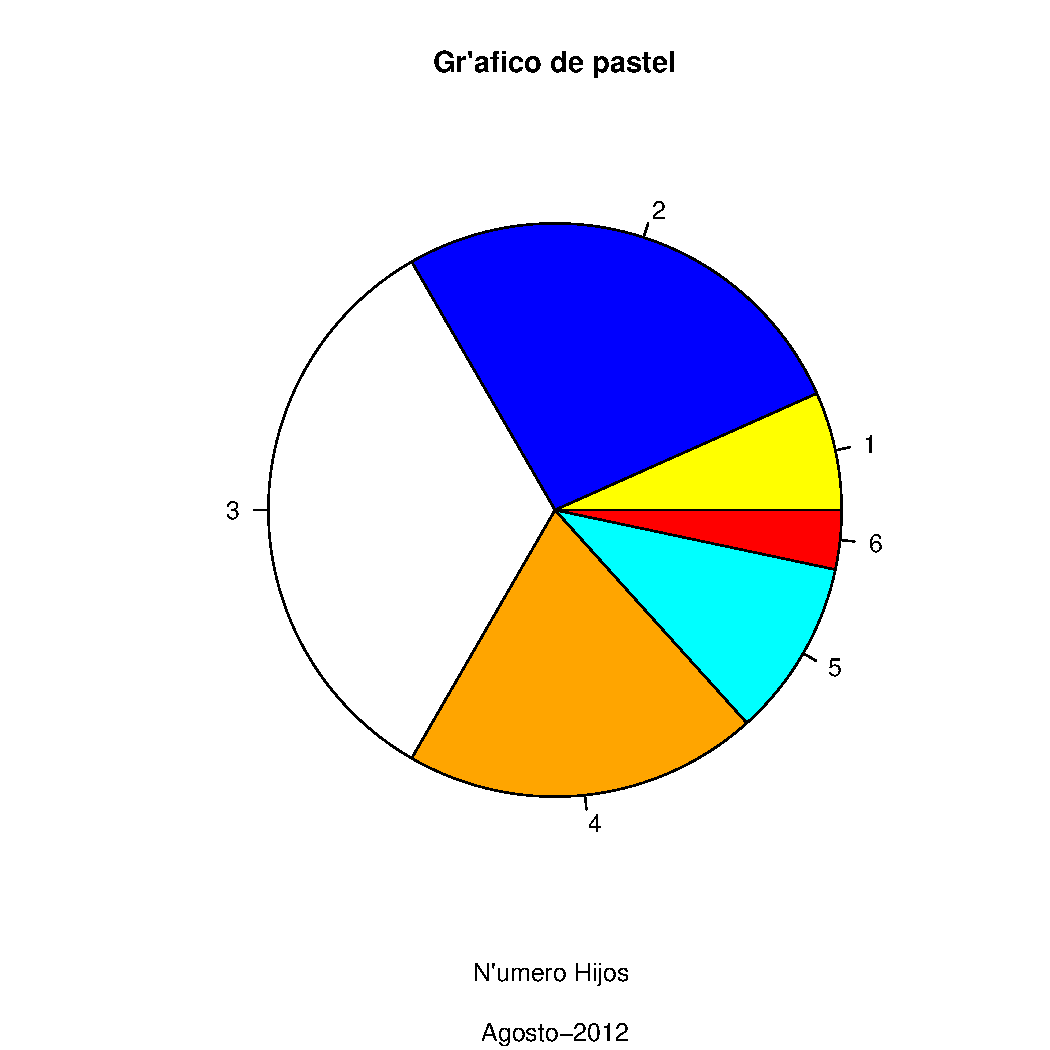
\includegraphics[width=\maxwidth]{figure/unnamed-chunk-9-2} 
\begin{kframe}\begin{alltt}
\hlcom{# Los colores se asignas dependiendo del orden en que han sido }
\hlcom{# especificados por names().Note con la instrucci\textbackslash{}'on radius se }
\hlcom{# especifica el tama\textbackslash{}~no de la figura, mientras m\textbackslash{}'as cerca de}
\hlcom{# uno (uno de menos uno) se encuentre m\textbackslash{}'as grande ser\textbackslash{}'a (el \textbackslash{}'angulo cambia).}
\end{alltt}
\end{kframe}
\end{knitrout}

11) Colocar valores num\'ericos en los sectores del gr\'afico
\begin{knitrout}
\definecolor{shadecolor}{rgb}{0.969, 0.969, 0.969}\color{fgcolor}\begin{kframe}
\begin{alltt}
\hlstd{n} \hlkwb{<-} \hlkwd{length}\hlstd{(frec)}
\hlstd{hoja} \hlkwb{<-} \hlkwd{data.frame}\hlstd{(frec);}
\hlstd{hoja}
\end{alltt}
\begin{verbatim}
##         Var1 Freq
## 1  Coca Cola    6
## 2      Pepsi    9
## 3 Salva Cola    5
\end{verbatim}
\begin{alltt}
\hlstd{etiq} \hlkwb{<-} \hlkwd{c}\hlstd{(}\hlkwd{paste}\hlstd{(hoja}\hlopt{$}\hlstd{Var1,} \hlstr{"-"}\hlstd{, hoja}\hlopt{$}\hlstd{Freq));}
\hlstd{etiq}
\end{alltt}
\begin{verbatim}
## [1] "Coca Cola - 6"  "Pepsi - 9"      "Salva Cola - 5"
\end{verbatim}
\begin{alltt}
\hlkwd{pie}\hlstd{(frec,} \hlkwc{main}\hlstd{=}\hlstr{"Gr\textbackslash{}'afico de pastel"}\hlstd{,} \hlkwc{labels}\hlstd{=etiq,} \hlkwc{col}\hlstd{=}\hlkwd{rainbow}\hlstd{(n),} \hlkwc{border}\hlstd{=}\hlnum{TRUE}\hlstd{)}
\end{alltt}
\end{kframe}
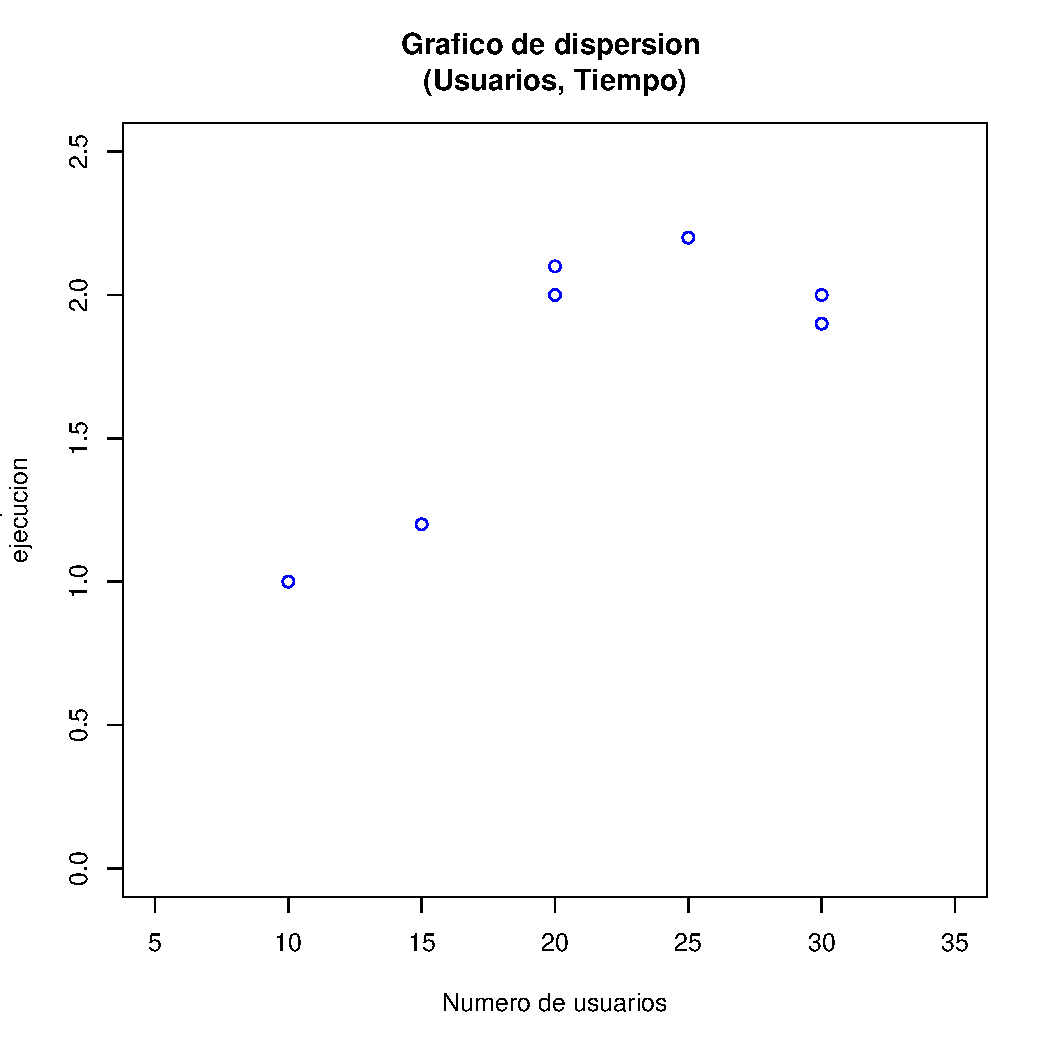
\includegraphics[width=\maxwidth]{figure/unnamed-chunk-10-1} 

\end{knitrout}

\end{document}
